\documentclass[12pt]{article}
\usepackage{enumerate, comment}
\usepackage{hyperref}
\usepackage{amsmath,amssymb,amsthm}
\usepackage{ wasysym }
\usepackage{ marvosym }
\usepackage{ textcomp }
\usepackage{xcolor}
\usepackage{graphicx}
\usepackage{epstopdf}
\usepackage{wrapfig}
\usepackage{epigraph}
\usepackage{tikz}
\usetikzlibrary{graphs}

\newcommand{\N}{\mathbb{N}}
\newcommand{\Z}{\mathbb{Z}}
\newcommand{\Q}{\mathbb{Q}}
\newcommand{\R}{\mathbb{R}}
\newcommand{\C}{\mathbb{C}}
\newcommand{\Aut}[1]{\ensuremath{ \aaut \left (#1 \right ) }}
\newcommand{\ins}[1]{\ensuremath{{#1}^{\mbox{in}}}}
\newcommand{\outs}[1]{\ensuremath{{#1}^{\mbox{out}}}}
\newcommand{\css}{\ensuremath{C_{ss} \left ( S_{g,p} \right) }}
\newcommand{\cn}{\ensuremath{C_{n}}}
\newcommand{\csn}{\ensuremath{C_{s,n}}}
\newcommand{\csnk}{{\ensuremath{C_{s,n}^{(k)}}}}
\newcommand{\outn}{{\ensuremath{ \oout(F_n)}} }
\newcommand{\nosep}{{\ensuremath{ \mathcal S^{\mbox{\tiny{nonsep}}}_n }}}
\newcommand{\coc}[1]{{\ensuremath{ \mathcal S^{\mbox{\tiny{coc}}}_{#1} }}}
\newcommand{\coco}[1]{{\ensuremath{ \mathcal {S^{\mbox{\tiny{coc}}}}^{(0)}_{#1} }}}
\newcommand{\ffn}{{\ensuremath{ \mathcal {FF}_n }}}
\newcommand{\sfn}{{\ensuremath{ \mathcal {SF}_n }}}
\newcommand{\sfno}{{\ensuremath{ \mathcal {SF}^{(0)}_n }}}


\DeclareMathOperator{\oout}{Out}
\DeclareMathOperator{\Mod}{Mod}
\DeclareMathOperator{\aaut}{Aut}
\DeclareMathOperator{\link}{link}
\newcommand{\cev}[1]{\reflectbox{\ensuremath{\vec{\reflectbox{\ensuremath{#1}}}}}}


\hypersetup{%https://preview.overleaf.com/public/hcstkvxftwfn/images/9aa75daac48baa3399aad3f640ea940279eb68d4.jpeg
  colorlinks=true,% hyperlinks will be black
  linkbordercolor=red,% hyperlink borders will be red
  pdfborderstyle={/S/U/W 1}% border style will be underline of width 1pt
}

\begin{document}


\section{Complexes of High Genus Separating Spheres}

%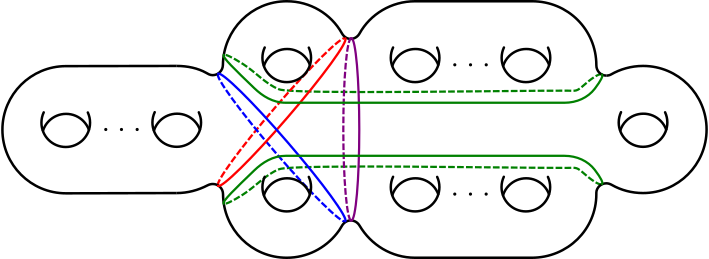
\includegraphics[width=.8\textwidth]{pentagon}
\noindent \textbf{Def of $C_n^{(k)}$, etc.}
\noindent \textbf{Sides are preserved}

\noindent \textbf{Def}
(Let $s \in C_n^{(k-1)}$ be a genus $k-1$ separating sphere.)
We say genus $k$ spheres $x$ and $y$ form a (genus $k-1$) sharing pair (for $s$) if there are genus $k$ spheres $a$ and $b$ and genus $k+1$ sphere $z$ such that 1) the induced subgraph of $C_n^{(k)}$ on $\{x,y,a,b,z\}$ is exactly the pentagon $x - z - y - b - a - x$, and 2) $x$ is the unique $k$ sphere disjoint from $a|_z$ in $C_z^{(k)}$. Similarly $y$ is unique $k$ sphere $b|_z$  in $C_z^{(k)}$.\\



\noindent \textbf{A sharing pair determines a unique genus $k-1$ sphere.}
Suppose $x,y$ form a sharing pair. Let $x-z-y-b-a-x$ be the corresponding pentagon.
Since $a|_z$ is disjoint from $x$, it must be that $a|_z$ is supported on a on a 1-handelbody $A \subset z^{in}$ such that $A \cup x^{in} \approx z^{in}$. 
Choose a maximal system $\Sigma$ of non-separating spheres in $z$ not intersectiong $x$ and $a|_z$.
Let $\alpha$ be the unique nonseparating sphere in $A$.
Consider a non-separating sphere $w$ in this system.
If any non-trivial loop $\gamma$ based at $w$ intersects both $\alpha$ and $x$ but not $a|_z$ then transvecting $x$ by $w$ along $\gamma$ gives infinitely many $k$-spheres in $z$ disjoint from $a|_z$, a contradition.
So it must be that $a|_z$ separates $\alpha$ from $x$.
Similarly $b|_z$ separates a nonseparating sphere $\beta \in \Sigma$ from $y$.
Since $a^{in}|_z$ and $b^{in}|_z$ are disjoint, they must separate $\alpha$ and $\beta$.
Hence there is a unique genus $k-1$ sphere in $z^{in}$ engulfing $\Sigma -\{\alpha, \beta\}$.\\

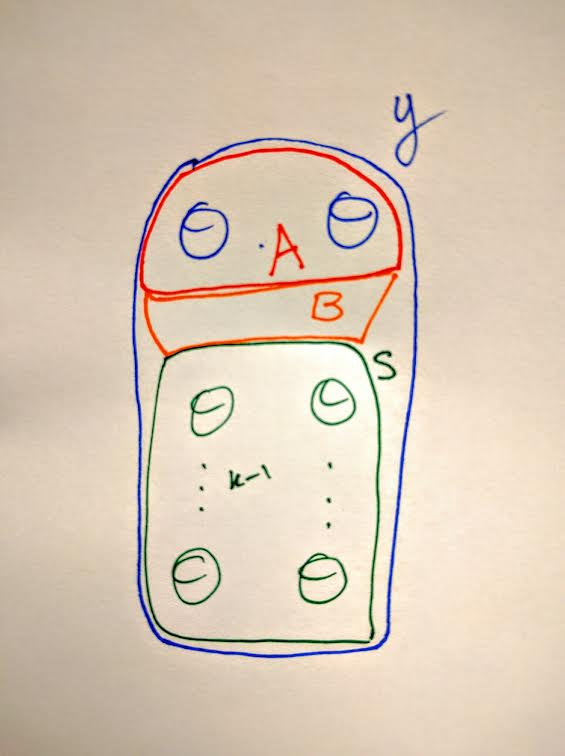
\includegraphics[width=.4\textwidth]{minintersect.jpg}

\noindent \textbf{Members of a sharing pair intersect minimally.}
Let $x,y$ be a sharing pair with $x-z-y-b-a-x$ the corresponding pentagon.
Let $s$ be the shared $k-1$ sphere.
Since $a|_z$ is disjoint from $x$, it must be that $a|_z$ is supported on a on a 1-handelbody $A \subset z^{in}$ such that $A \cup x^{in} \approx z^{in}$. 
Since $A-a^{in}$ is simply connected and $x$ does not intersect $a$,
$x$ must not intersect $\partial A$.
We can take a representatives such that $y \cup y^{in}$
is partitioned into $s\cup s^{in}$, the handebody $A$, and $B \approx D^2 \times I$ such that $D^2 \times \{0\}$ is a disk in $s$ and $D^2 \times \{1\}$ is a disk in $\partial A$.
Since $x$ intersects $y$, but not $\partial A$ or $s$, it must be that $x$ intersects $B$ in a disk.\\

\noindent \textbf{Sharing Pairs Preserved}
Let $\phi \in \Aut {C_n^{(k)}}$. If $x,y$ form a sharing pair, then $\phi(x),\phi(y)$ form a sharing pair. By combinatorial definition.\\
\\

\noindent \textbf{Every $k-1$ sphere admits a sharing pair for $n\geq 3k$}

As below.

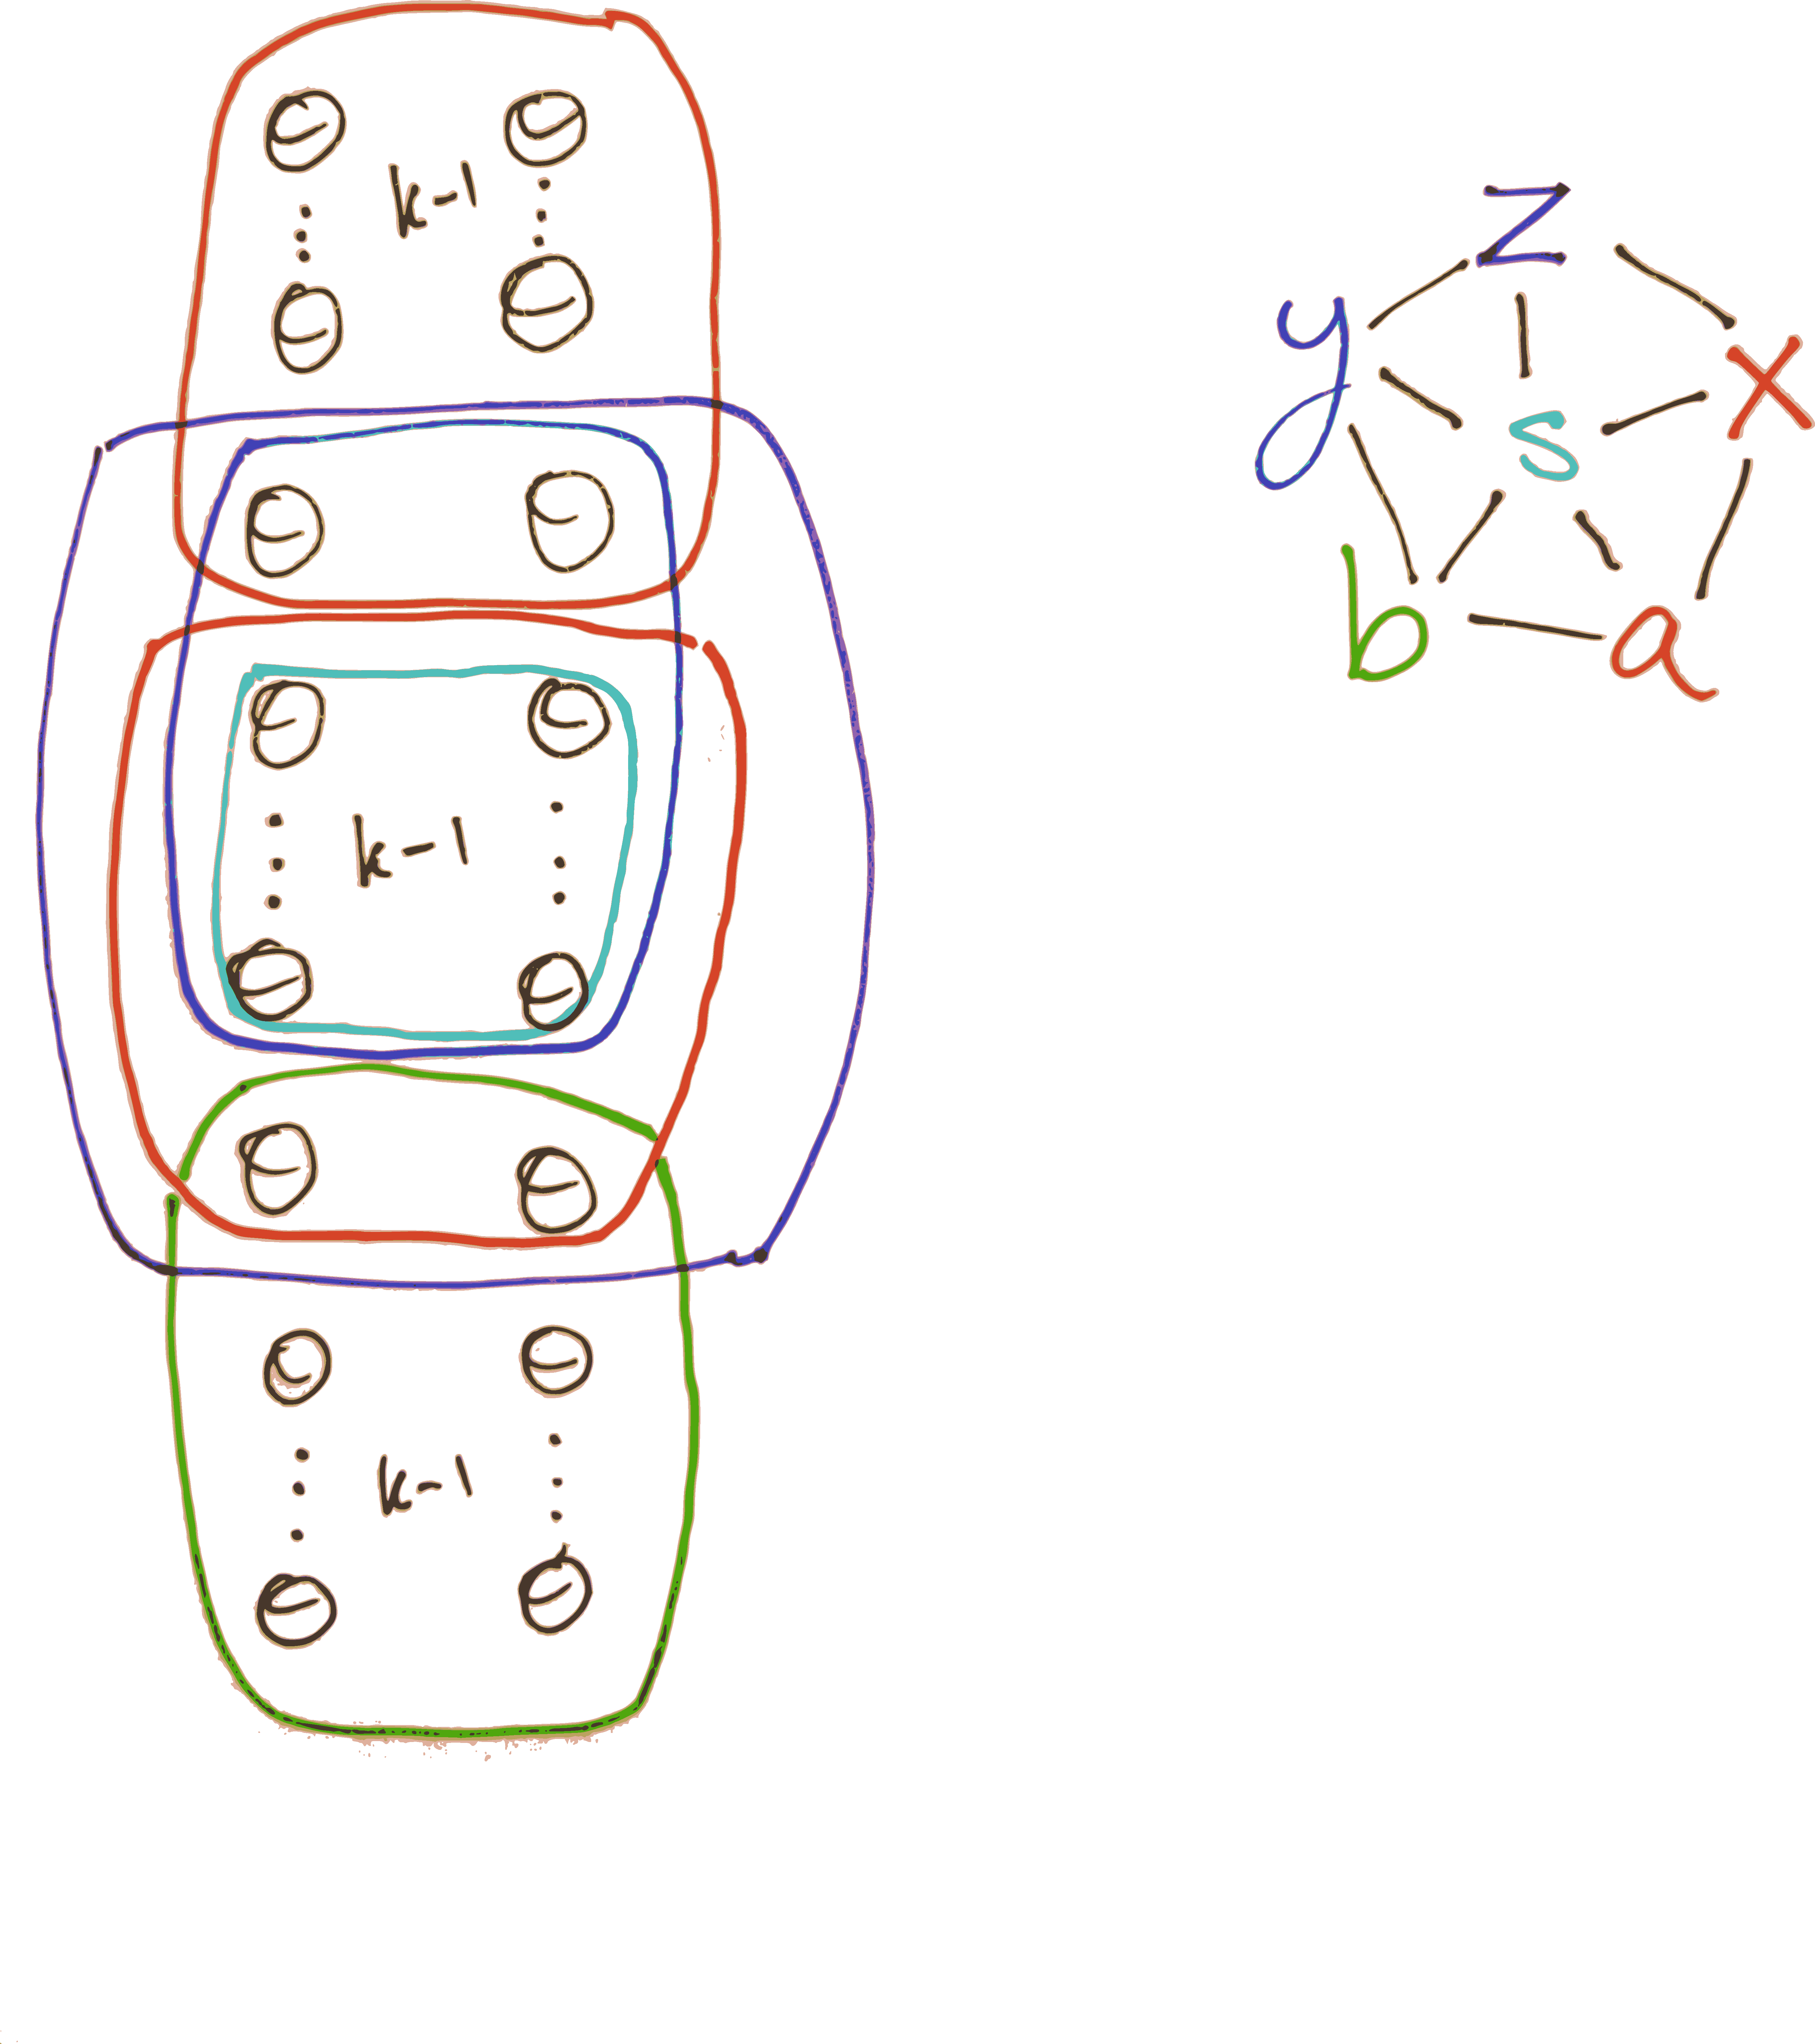
\includegraphics[width=.6\textwidth]{spherepentagon}

\noindent \textbf{Extend  by sharing pairs.}
$ \Phi: \Aut{C_n^{(k)}} \to \Aut{C_n^{(k-1)}}$\\
For genus $k-1$ sphere $s$, choose a sharing pair $\{x,y\}$ for $s$.
Define $\Phi(\phi)(s)$ as the $k-1$ sphere specified by $\{\phi(x), \phi(y)\}$.\\

\noindent \textbf{$\Phi$ is well defined}\\


We say $\{x,y,z\}$ form a sharing triple if there is  a genus $k-1$ sphere $s$ such that any two of $\{x,y,z\}$ form a sharing pair sharing $s$.


\noindent \textbf{Sharing triples are preserved by $\phi \in \Aut {C_n^{(k)}}$}
Observe that the triple $\{x,y,z\}$ is contained in a $k+2$ sphere, namely $w \approx \partial \left ( \overline{x^{in}  \cup  y^{in} \cup z^{in}} \right )$, and no smaller sphere.
So $\{\phi(x),\phi(y),\phi(z)\}$ are pairwise sharing pairs in $k+2$ sphere
$\phi(w)$.
Assume to the contrary that sphere $w'$ contains $\phi(x)$,  $\phi(y)$, and $ \phi(z)$
and has genus less than $k+2$.
Then there is a sphere intersecting $\phi(w)$ but not $\phi(x), \phi(y)$, or $\phi(z)$, contradicting that $w$ intersects no sphere not intersecting $x,y,$ or $z$.
So $\phi(w)$ is the minimal genus sphere containing
$w'=\overline{\phi(x)^{in} \cup \phi(y)^{in} \cup \phi(z)^{in}}$.
Since sharing pairs intersect minimally,  it must be that $w'$ is a sphere, and so
$\phi(w) \approx w'$.
Observe further that the triple partitions their complement in $w'$ into 7 connected regions, a la triple-Venn-diagram.
Consider the genera of these regions.
The regions' genrera total $k+2$.
Each pair in $\{\phi(x),\phi(y),\phi(z)\}$ must have genus $k-1$.
The regions in  $\phi(x)$ (sim. $\phi(y),\phi(z)$) must have genera summing to $k$.
The only solution requires the genus of $\phi(x)^{in} \cap \phi(y)^{in}\cap \phi(z)^{in} $ be $k-1$. Then $\phi(s) \approx \partial \left ( \overline {\phi(x)^{in} \cap \phi(y)^{in}\cap \phi(z)^{in} } \right ) $ is shared by $\{\phi(x),\phi(y),\phi(z)\}$.\\
\\

Let $s$ be a genus $k-1$ sphere.
Form a complex $P_s$ of sharing pairs that represent $s$ as follows:
The vertices of $P_s$ are all sharing pairs that shair $s$.
Two sharing pairs are joined by an edge in $P_s$ if they have a common member, i.e form a sharing triple. The above implies\\

\noindent \textbf{$\phi \in \Aut {C_n^{(k)}}$ induces $\phi_\ast \in \Aut {P_s}$}\\
\\

\noindent \textbf{(Putnam's Lemma)} Let group $G$ with generators $H$ act on simplicial set $X$. Fix a basepoint $v \in X^{(0)}$. 
If 
\begin{enumerate}
\item for all $v' \in X^{(0)}$ the orbit $G\cdot v$ intersects the connected component of $v'$ in $X$ and 
\item for all $h \in H^{\pm}$ there is some path from $v$ to $h\cdot v$ 
\end{enumerate}
then $X$ is connected.\\

We will use Putnam's Lemma with the complex $P_s$ and the group $G$ of outer automorphisms respecting the splitting given by $s$.\\



\noindent \textbf{$P_s$ is connected}\\
\\
Fix a maximal system $\Sigma$ of nonseparating spheres with every sphere disjoint from $s$, so there are $n-k+1$ spheres $\alpha_1, \ldots, \alpha_{n-k+1}$ in $s^{out}$ 
and $k-1$ spheres $\beta_1,\ldots \beta_{k-1}$ in $s^{in}$.
Assign an orientation to every sphere of $\Sigma$ and let $M_\Sigma$ be manifold obtained by removing a regular neighborhood of the spheres of $\Sigma$.
Thus the components of $\partial M_\Sigma$ are labeled $\alpha^{\pm}_i$ or $\beta^{\pm}_i$
and we obtain $M_n$ by gluing $\alpha^+_i$ to $\alpha^-_i$ and 
$\beta^+_i$ to $\beta^-_i$.

Observe that we can construct a genus $k$ sphere containing $s$ as follows.
Choose a path $\gamma$ from a point of $s$ to a genus 1 sphere $a \subset s^{out}$. 
Then the boundary of a regular neighborhood of $s^{in} \cup \gamma \cup a^{in}$
is a genus $k$ sphere.
Moreover any genus $k$ sphere $w$ engulfing $s$ can be represented uniquely by a genus 1 sphere $a$  in $w^{in} - s^{in}$ and an arc from $a$ to $s$ disjoint from $s^{in}$ and $a^{in}$.

Let $x$ (resp. $y$) be the unique genus $k$ sphere in $M_\Sigma$ engulfing exactly $\{\beta_i^{\pm}\}_i$ and $\alpha^{\pm}_1$ (resp. $\alpha^{\pm}_2$).
Let $v=\{x,y\}$.\\


\noindent \textbf{$G$ acts transitively on sharing pairs of $s$}\\


(This should probably be a much earlier lemma)
We claim $G \cdot v = P_s^{(0)}$.
Take any sharing pair $\{x',y'\}$.
Fix a maximal system $\Sigma'$ of nonseparating spheres disjoint from $x'$ and $y'$.
Then there are $\{\beta'_i\}_{i=1}^{k-1}$ engulfed by both $x$ and $y$ and $\{\alpha'_i\}_{i=1}^{n-k+1}$ spheres such that $x'$ engulfs $\alpha'_1$ and $y'$ engulfs $\alpha'_2$.
Then a homeomorphism $M_{\Sigma'} \to M_{\Sigma}$ sending ${\alpha'}^\pm_i \to \alpha^\pm_i$
 and ${\beta'}^\pm_i \to \beta^\pm_i$ is realized by the outer automorphism giving the action on the $\pi_1$ bases dual of $\Sigma '$ to that of $\Sigma$.
Then the image of $x'$ is $x$ and of $y'$ is $y$.\\
 
 
\noindent \textbf{$v$ is connected to its image under a Whitehead move}\\
 
A generating set for $G$ is given by:
\begin{enumerate}
\item $a$-rotation permuting $(a_1 \cdots a_{n-k+1})$: takes $v$ to an adjacent sharing pair
\item $a$-transposition $(a_1 a_2)$: fixes $v$
\item $a$-inversion $a_1 \mapsto a_1^{-1}$: fixes $v$
\item $a$-transvection $a_1 \mapsto a_1a_2$:
There is a length 4 path in $P_s$ from $v$ to its image for $n\geq k+3$

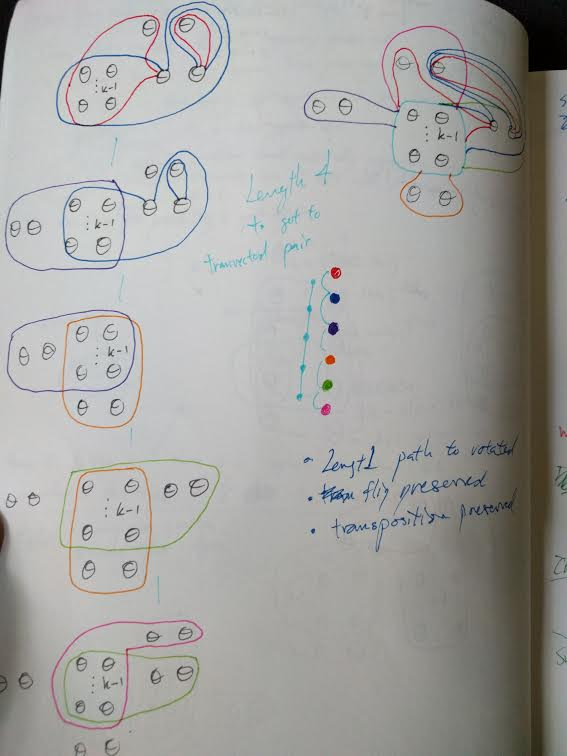
\includegraphics[width=.6\textwidth]{transvect.jpg}

\item $b$-rotation permuting $(b_1 \cdots b_{k-1})$: fixes $v$
\item $b$-transposition $(b_1 b_2)$: fixes $v$
\item $b$-inversion $b_1 \mapsto b_1^{-1}$: fixes $v$
\item $b$-transvection $b_1 \mapsto b_1b_2$: fixes $v$
\end{enumerate}

\noindent \textbf{$\Phi$ is well defined}\\
Given two sharing pairs for $s$ there is a path between them.
Adjacent sharing pairs for $s$ in $P_s$ determine the same $k-1$ sphere under $\phi$.
So $\Phi(\phi)(s)$ is independent of the sharing pair used to define $s$.\\


\noindent \textbf{$\Phi$ is an isomorphism for $n \geq \max\{3k ,k+3\}$}\\

We claim that the restriction $\Aut{C^{(k-1)}_n} \stackrel{\Psi}{\to} \Aut{C^{(k)}_n}$ is the inverse homomorphism to $\Phi$.
Certainly $\Psi \circ \Phi$ is by definition the identity on $\Aut{C^{(k)}_n}$.
Consider $\phi^{-1}\Phi(\Psi(\phi))$ for $\phi \in \Aut{C^{(k-1)}_n}$.
This is an automorphism fixing all genus $k$ or greater spheres. 
But since any sharing pair for a genus $k-1$ sphere is fixed, so $\phi^{-1}\Phi(\Psi(\phi))$ is the identity.\\


\noindent \textbf{ $\Aut{C^{(k)}_n} \cong \outn$ for $n \geq \max\{3k ,k+3\}$}\\

We induct on $k$.
The inductive step is given above.
It thus suffices to show that $\Aut{C^{(1)}_n} \cong \outn$. We need only see that $\Aut{C^{(1)}_n} \cong \Aut{C_n}$.
Given $ \phi \in \Aut{C^{(1)}_n}$ extend to $ \Phi(\phi): \Aut{C_n} \to \Aut{C_n}$
by for any non-separating sphere $\alpha$ choosing a genus 1 sphere $s$ engulfing $\alpha$ and defining $\Phi(\phi)(\alpha)$ to be the non-separating sphere engulfed by $\phi(s)$.
To see that this is well defined, recall that $\alpha$ non-separating sphere corresponds to an HNN extension $F_n=A\ast_t$. Then a genus 1 sphere engulfing $\alpha$ is a splitting $A \ast \langle x \rangle$ for some $x \in F_n$ so that the unique HNN extension compatible with $\phi_\ast(A) \ast \langle \phi_\ast(x) \rangle$ and must be $\phi_\ast(A) \ast_t$ which is clearly independent of the choice of $x$ and so gives an automorphism of $C_n$.



Observe that restriction 
$\Psi: \Aut{C_n} \to \Aut{C^{(1)}_n}$
is the inverse homomorphism.
Certainly $\Psi \Phi$ is by definition the identity.
Consider $\phi \in \Aut{C_n}$ and $\phi'=\phi^{-1} \Phi(\Psi(\phi))$.
Then $\phi'$ fixes all separating spheres.
But if $\alpha \neq \beta$ are nonseparating spheres then there is a $\phi'$-fixed genus 1 sphere engulfing $\alpha$ and intersecting only $\beta$ exactly once, so $\phi'(\alpha) \neq \beta$.



\begin{comment}

\noindent \textbf{Notations}
$\csn$ is the complex of embedded separating spheres in $M_n$.
$\csnk$   is the complex of embedded separating spheres genus $k$ or greater.
For a separating sphere $x$ of genus $< \frac n 2$, we write $\ins x$ for the lower-genus side of $M_g - x$.\\
\\
\noindent \textbf{Def}
Let $k!!!!< \frac n 2$.
We say that genus $k+1$ separating spheres $x,y \in \csn$ form a $k$-\emph{sharing pair} if they intersect once and there are representatives such that $\partial ( \ins x \cap \ins y )$ is genus $k$.\\
\\
\noindent \textbf{Def}
Let $x \in \csn$. 
Define $C(x)$ as the simplicial complex of homotopy classes of spheres and loops in $\ins x$ with a simplex for every collection of homotopy classes that have simultaneously disjoint representatives.\\
\\
\noindent \textbf{Lemma} C(x) is a flag complex.\\
\\
\noindent \textbf{Remark} 
There is a projection map $\pi_x: \csn \to 2^{\mbox{vertices } C(x)}$.
Observe that if $z \in \csn$  lies in $\outs x$ then $\pi_x(z)=\varnothing$.
If $z$ lies in $\ins x$ then we get a single vertex of $C(x)$.
Otherwise a $z$ representative intersects $\ins x$ in a collection of essential disks and annuli with boundaries in $x$. By homotoping the 


\noindent \textbf
{Remark}
Automorphisms of $\csnk$ preserve the adjacency graphs of simplices since the adjacency graph is the corresponding graph of groups in outer space.\\
Also preserves the genus as the link of a separating sphere $s$ is the join of the complex of spheres of the components of the compliments of $s.$\\

\\
\noindent \textbf{Lemma} $[(D,\partial D), (H_g,\partial H_g)] \twoheadrightarrow [S^2, M_g]$.  (I mean classes of embeddings...)\\
\\
\noindent \textbf{Cor} $\Mod(M_n)$ acts transitively on non-separating spheres, sim. spheres genus $k$\\

\noindent \textbf{Theorem} $\Aut \csnk \cong \outn$ for $n > f(k)$.\\
\\
Proof is by induction on $k$.\\
\\
Base case $C_{s,n}$.
Extend $\phi \in \Aut \csn$ to $\tilde \phi \in \Aut \cn$ as follows.
Let $s$ be non-separating.
Consider a reduced simplex $\Sigma$ containing $s$ such that $M_g \setminus \Sigma$ is a 3-sphere with $2n$ balls removed. 
Let $t$ be a sphere separating $s_+$ and $s_-$ from the other boundary spheres of $M_g \setminus \Sigma$.
Then $t$ is genus 1.
Then $\phi (t)$ is genus 1 and contains a unique non-separating sphere $s'$.
Define $\tilde \phi(s)=s'$.

Well-definedness: Observe that there are infinitely many choices for $t$.\\

\noindent \textbf
{Definition}
Let $x$ and $y$ be genus 1 separating spheres. We say that $x$ and $y$ are a \emph{sharing pair} if there is a non-separating curve in $\cev x \cap \cev y$.\\


\noindent \textbf{Lemma}
Let $x$ and $y$  be genus 1 spheres in $\cev z$ where $z$ is a genus 2 sphere. Then $x$ and $y$ share a non-separating curve iff genus 1 curve $w$ such that the induced subgraph on $w,x,y,z$ is exactly \\
\tikz \graph  {
x--w,
z--y,
x--z,
w--y
};

\noindent \textbf{Proof}
$(\Rightarrow)$
Suppose that $x$ and $y$ are genus 1 spheres in $\cev z$ such that they share non-separating sphere $v$.
Represent them in the disk model as curves bounding disks in a genus 2 surface with boundary component $z$ (red).

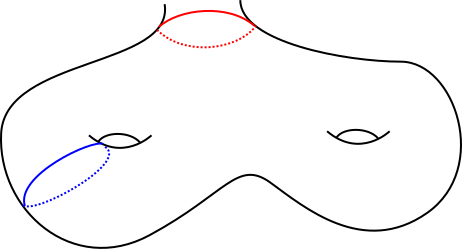
\includegraphics[width=.5\textwidth]{sharepairA}

Since $x$ and $y$ must engulf $v$ we can represent them as follows. 
Take parallel copies on either side of $v$ and join them into one disk by the adding the boundary of a regular neighborhood of a simple arc $a$ (light green) connecting the parallel copies.
But we are considering these arcs up to isotopy in the handlebody, which are totally determined by a winding number about the remaining genus of $\cev z \setminus v$.
 
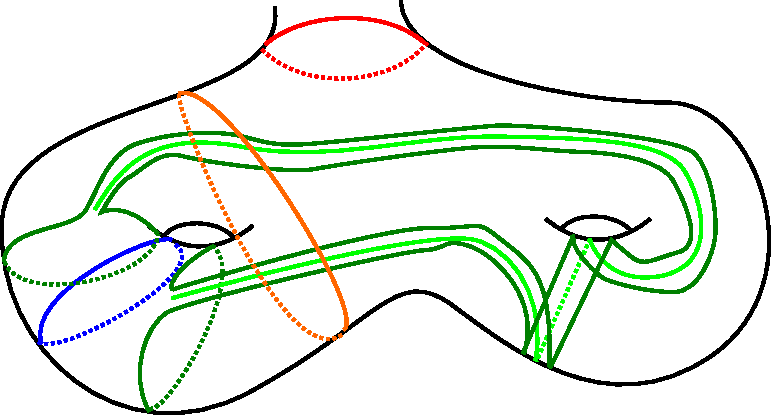
\includegraphics[width=.5\textwidth]{sharepairB}

\end{comment}
\newpage
\section{False Free Factor Complex Attempt}


Let $F_n$ be the rank $n$ free group.
If $F_n$ can be expressed as the internal free product of subgroups $A,B \leqslant F_n$, then $A$ and $B$ are \emph{free factors} of $F_n$.
The free factor complex $\mathcal {FF}_n$ is the simplicial complex with a $k$-simplex given by conjugacy classes of length $k+1$ chains of proper free factors.
The purpose of this note is to give a new proof of the following theorem of Bestvina and Bridson \cite{bridson}.\\
\\
\noindent \emph{Theorem 1.} (Bestvina--Bridson) For $n \geq 3$ we have $\Aut{\ffn} \cong \outn$.\\

Let $M_{n}$ be the connect sum of $n$ copies of  $S^1 \times S^2$, with the convention that $M_0 =S^3$.
We will consider a series of simplicial complexes where the simplices correspond to collections of spheres in 
$M_n$.

When discussing spheres or submanifolds of $M_n$ below, we will always mean their homotopy classes.
We define the following three simplicial complexes related to the free factor complex:
\begin{enumerate}[$\cdot$]
\item
Let $\nosep$ be the simplicial complex with $k$-simplices specified by $k+1$ disjoint nonseparating spheres in $M_n$.
\item
Let $\coc n$ be the subcomplex of $\nosep$ with simplices given by collections of spheres which are coconnected (i.e. have connected complement) in $M_n$.
\item
Let $\sfn$ be the barycentric subdivision of the $(n-2)$-skeleton of $\coc n$. Thus vertices of $\sfn$ are coconnected sets of at most $n-1$ spheres, and simplices are given by chains of proper subsets.
\end{enumerate}
For a simplex $\Sigma_0 \subset \cdots \subset \Sigma_k$ of $\sfn$, we obtain a simplex of $\ffn$ by the (conjugacy class of) free factors $$\pi_1(M_n-\Sigma_k,\ast) \leqslant \cdots \leqslant \pi_1(M_n-\Sigma_0,\ast)$$ so that as posets $\sfn \to (\ffn)^{op}$ is a quotient map.
\\
\noindent \emph{Theorem 3.} For $n \geq 3$ we have
$\Aut{\sfn} \cong \Aut{\coc n} \cong \Aut{\nosep}$.\\
\\
Pandit \cite{pandit}.\\
\\
\emph{Theorem 4.} (Pandit) For $n \geq 3$ we have $\Aut{\nosep} \cong \outn$.\\
\\
Our first goal is to show that $\Aut{\sfn} \cong \Aut{\coc n}$.

Let $M_{n,s}$ be the manifold $M_n$ with interiors of $s$ disjoint closed  balls removed. We call $n$ the \emph{genus} of $M_{n,s}$. If $\Sigma$ is a set of disjoint embedded spheres of $M_{n,s}$, we will denote by $M_{n,s}|\Sigma$ the manifold $M_{n,s}$ cut along $\Sigma$.\\
\\
\noindent \emph{Lemma 5.} Automorphisms of $\sfn$ preserve the cardinality of sets of spheres.
\begin{proof}
We induct downward on the cardinality of sets of spheres.
We claim as a base case that a set of spheres $\Sigma \in \sfno$ has $n-1$ spheres if and only if
it is adjacent to finitely many sets of spheres in $\sfn$, namely, the proper subsets of $\Sigma$.
If $\Sigma \in \sfno$ has fewer than $n-1$ spheres, then
$M_n|\Sigma$ has genus $k \geq 2$.
The complex of coconnected nonseparating spheres of $M_n|\Sigma$ is isomorphic to $\coc k$, which is infinite.
Choose any nonseparating sphere $a$ of $M_n|\Sigma$. Then $\Sigma \cup \{a\}$ is coconnected in $M_n$ and adjacent to $\Sigma$ in $\sfn$.

Assume that automorphisms of $\sfn$ preserve the size of sets of spheres with at least $k+1$ spheres. 
Let $A_k \subset \sfno$ be the sets of spheres of $\sfn$ with $k$ or fewer spheres.
A set of spheres $\Sigma \in A_k$ has $k$ spheres if and only if $\link(\Sigma) \cap A_k$ is finite.
By hypothesis automorphisms of $\sfn$ preserve $A_k$ and its complement, so must preserve the class of sets of $k$ spheres.
\end{proof}

We now prove the first isomorphism of Theorem 3.\\

\noindent \emph{Proposition 6.} For $n\geq 3$ we have $\Aut \sfn \cong \Aut{\coc n}$.
\begin{proof}
As $\sfn$ is the barycentric subdivision of the $n-2$ skeleton ${\coc n}^{(n-2)}$, there is a natural map 
$$\Phi: \Aut{\coc n} \to \Aut{\sfn}.$$ We will construct the inverse. Let $\phi \in \Aut{\sfn}$.
The vertices of $\sfn$ are the simplices of $\coc n$ with dimension $n-2$ or less.
Then $\phi$ induces a bijection $\phi_\ast$ of simplices of ${\coc n}^{(n-2)}$. 
By Lemma 5 we have $\phi_\ast$ preserves the dimension of simplices, so $\phi_\ast$ is an automorphism of ${\coc n}^{(n-2)}$.

It remains to see that $\phi_\ast$ also preserves $n-1$ simplices.
To see this we will show that a collection of $n$ disjoint separating spheres $\Sigma$ form a simplex in $\coc n$ if and only if 
$$\coco n \cap  \left ( \bigcap_{x \in \Sigma} \link(x) \right )$$
is finite.
Note that if $\Sigma$ is a coconnected set of $n$ spheres, then $M_n|\Sigma$ is homeomorphic to $M_{0,2n}$. Then $\pi_2(M_n|\Sigma)$ is the free abelian group generated by any $2n-1$ of the balls, and an embedded sphere must be degree at most 1 over any generator.
There are thus finitely many  embedded spheres of $M_n|\Sigma$. 
Then $\bigcap_{x \in \Sigma} \link (x)$ contains finitely many vertices of $\coc n$.
Conversely suppose $\Sigma$ is a non-coconnected set of $n$ disjoint spheres.
Then $M_n|\Sigma$ has a component $M'$ with genus at least one and at least two boundary spheres.
Choose a non-separating sphere $x$ of $M'$, a boundary sphere $y$, and a loop $\alpha$ based at $y$ intersecting $x$ once. The push map of $x$ along $\alpha$ produces a collection $A$ of infinitely many spheres of $M_n$. Each $a \in A$ is nonseparating in $M' \subset M|\Sigma$, so $\{a,x\}$ is coconnected for any $x \in \Sigma$. Then  $A\subset \bigcap_{x \in \Sigma} \link (x)$.
Thus $\phi_\ast$ must also preserve $n-1$ simplices and gives a simplicial automorphism of $\coc n$.
Then $\phi \mapsto \phi_\ast$ gives the inverse homomorphism to $\Phi$.
\end{proof}



Call a collection of $m$ disjoint spheres $\Sigma \subset {\coc n}^{(0)}$ a \emph{bounding $m$-tuple} (pair, triple, etc.) if $\Sigma$ is not coconnected but every proper subset of $\Sigma$ is. 
The genus of the bounding tuple is the smaller of the genera of the two components of $M_n|\Sigma$.
The following lemma shows we can detect the genus combinatorially.\\
\\
\noindent \emph{Lemma 7.} 
The link of a genus $k$ bounding $m$-tuple of $\coc n$ is isomorphic to the join $\coc{k} \ast \coc{n-k-m+1}$.
\begin{proof}
Consider $\Sigma \subset {\coc n}^{(0)}$ a bounding $m$-tuple with genus $k$.
Then $M_n|\Sigma$ has two components, $R_1 \cong M_{k,m}$ and $R_2 \cong M_{n-k-m+1,m}$.
Let $V_i$ be the complex of coconnected nonseparating spheres in $R_i$.
So $V_1 \cong {\coc {k}}$ and $V_2 \cong \coc {n-k-m+1}$.
We claim that $\link(\Sigma)$ is the join $V_1 \ast V_2$.
Certainly $\link(\Sigma) \subset V_1 \ast V_2$.
Consider sets of spheres $\Sigma_i$ giving simplices of $V_i$. 
The $R_i|\Sigma_i$ are connected. $M_n|(\Sigma_1 \cup \Sigma_2)$ is $R_1|\Sigma_1$ and $R_2|\Sigma_2$ glued along $\Sigma$, and hence connected. So $\Sigma_1\cup \Sigma_2$ must be coconnected in $M_n$ and the join $\Sigma_1 \ast \Sigma_2$ lies in $\link(\Sigma)$.
\end{proof}

We now prove the second isomorphism of Theorem 3.\\

\pagebreak[3]
\noindent \emph{Proposition 8.} For $n\geq 3$ we have $\Aut{\coc n} \cong \Aut{\nosep}$. \nopagebreak
\begin{proof}
Restriction gives a natural map 
$$\Phi: \Aut{\nosep} \to \Aut{\coc n}.$$ 
We will construct the inverse. Observe that since $\coco n = {\nosep}^{(0)}$ any $\phi \in \Aut{\coc n}$ induces a set map $\phi_\ast$ of ${\nosep}^{(0)}$. 
If $\phi_\ast$ is a simplicial automorphism, then $\phi \mapsto \phi_\ast$ is the inverse homomorphism to $\Phi$. 
As $\nosep$ is a flag complex (Lemma 3 of \cite{souto}), it will suffice to show that $\phi_\ast$ sends pairs of disjoint spheres to pairs of disjoint spheres. 
Disjoint nonseparating spheres form a bounding pair if and only if they are not adjacent in $\coc n$.
So it suffices to show that $\phi$ preserves bounding pairs of $\coc n$.
We will demonstrate this through the stronger result that $\phi$ preserves the set of genus $k$ bounding $m$-tuples.

\medskip \noindent \emph{Case 1.} Suppose $\Sigma$ is a genus $k$ bounding $m$-tuple with $m>2$. Any $\Sigma' \subset {\coc n}^{(0)}$ is a bounding $m$-tuple if and only if $\Sigma'$ does not span a simplex in $\coc n$, but every proper subset of $\Sigma'$ does. Hence if $\phi \in \Aut{\coc n }$, then $\phi(\Sigma)$ is a bounding $m$-tuple. By Lemma 7, $\link(\Sigma)$ is isomorphic to $\coc {k} \ast \coc{n-k-m+1}$. We can determine $k$ by the maximal simplex dimension on the sides of the join. Then $\phi(\Sigma)$ is also genus $k$.

\begin{figure}[b!]
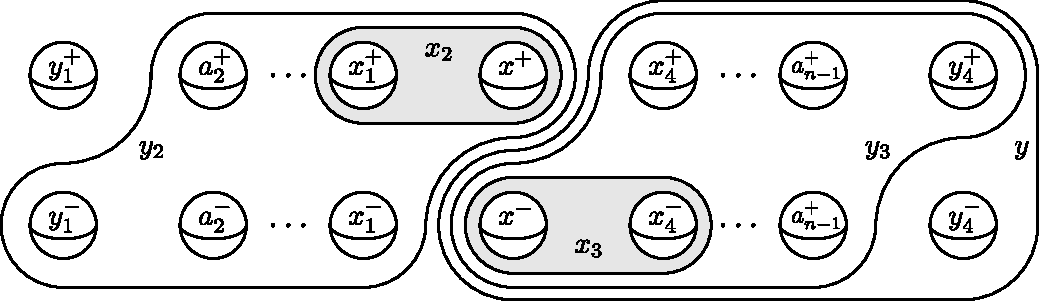
\includegraphics[width=\textwidth]{spheresagain.pdf}
\caption{
The manifold $M_n|\{a_i\}_{i=1}^n$ is $S^3$ with $2n$ balls removed.
We obtain $M_n$ by again identifying the spheres with $+$ and $-$ labels via a vertical reflection.
The spheres $\Sigma'=\{x_i,y_i\}_{i=1}^4$ are such that $M_n|\Sigma'$ contains $x$ and $y$ in disjoint copies of $M_{0,4}$. The $M_{0,4}$ containing $x$ (identify $x^+$ and $x^-$) is shaded. The $M_{0,4}$ containing $y$ is the exterior of $y_2$ and $y_3$.
}
\label{fig:spherediagram}
\end{figure}

\medskip \noindent \emph{Case 2.} Suppose $\Sigma=\{x,y\}$ has $m=2$ spheres.
Choose a collection $\Sigma'$ of disjoint nonseparating spheres such that  there are two separate components of $M_n|\Sigma'$ homeomorphic to $M_{0,4}$ and containing $x$ and $y$ respectively.
We can construct $\Sigma'$ as follows.
$M_n|\Sigma$ has two components, homeomorphic to $M_{k,2}$ and $M_{n-k-1,2}$.
So we have a set of spheres $\{a_i\}_{i=1}^n$ coconnected in $M_n$ disjoint from $y$ with $a_{k+1}=x$.
Choose $x_2,x_3,y_2,y_3$ as shown in figure \ref{fig:spherediagram} and relabel $a_1=y_1$, $x_{1}=a_k$, $x_4=a_{k+2}$, $y_4=a_n$. 
Then 
$\{x_1,\ldots, x_4\}$ (resp. $\{y_1, \ldots, y_4\}$ are the boundary spheres of a component of $M|\Sigma'$ homeomorphic to $M_{0,4}$ and containing $x$ (resp. $y$).
Further $\{x,x_1,x_2\}$ and $\{x,x_3,x_4\}$ are genus 0 bounding triples. Let $\Sigma' =\{x_i,y_i\}_{i=1}^4$.



By Case 1 we have that $\{\phi(x_1), \ldots, \phi(x_4)\}$ is a genus 0 bounding $4$-tuple and $\{\phi(x),\phi(x_1),\phi(x_2)\}$ and $\{\phi(x),\phi(x_3),\phi(x_4)\}$ are genus 0 bounding triples. 
So $\{\phi(x_1), \ldots, \phi(x_4)\}$ define a component of $M|\Sigma'$ homeomorphic to $M_{0,4}$ and containing $\phi(x)$.

If $\{x_1, \ldots, x_4\} \neq \{y_1, \ldots, y_4\}$ then 
 $\phi(x)$ and $\phi(y)$ lie in disjoint $M_{0,4}$ homeomorphic components of $M|\phi(\Sigma')$.
Then  $\phi(x)$ and $\phi(y)$ are are disjoint. They are also not adjacent in $\coc n$, so they are bounding a pair.

Suppose $\{x_1, \ldots, x_4\} = \{y_1, \ldots, y_4\}$.
Then $n=3$ and $M_3|\{x_i\}_{i=1}^4$ is homeomorphic to two copies of $M_{0,4}$.
As $x,y$ form a bounding pair, the bounding triples must be
$\{x,x_1,x_2\}$, $\{x,x_3,x_4\}$, $\{y,x_1,x_2\}$, and $\{y,x_3,x_4\}$.
Then the $\phi$ image of these triples are
bounding triples giving $\phi(x)$ and $\phi(y)$ contained in disjoint $M_{0,4}$.
Then $\phi(x)$ and $\phi(y)$ are disjoint and must form a bounding pair.
\end{proof}

\newpage
\section{Free Factor Complex}


Fix an identification $F_n \stackrel{\cong}{} \pi_1(M_n,\ast)$.
We take the convention that $\mathcal{FF}_k$ is empty for $k<2$ and an infinite disconnected set for $k=2$.

\noindent \emph{Lemma 1.} The link of a rank $k$ free factor is isomorphic to the join $\mathcal{FF}_{k} \star \mathcal{FF}_{n-k}$.\\
\\
Let $A$ be a rank $k$ free factor.
Then the vertices of the link of $A$ are the proper free subfactors and superfactors of $A$.
The subfactors of $A$ form a complex $\mbox{link}_-(A)$ isomorphic to the free factors of $F_k$.
By the lattice isomorphism theorem, we have that the superfactors of $A$ from a complex $\mbox{link}_+ (A)$ isomorphic to the free factors of $F_n/A \cong F_{n-k}$.\qed \\
\\

\noindent \emph{Lemma 2.} An automorphism $\phi \in \Aut \ffn$ preserves the rank of free factors.\\
\\
We first demonstrate that the class of rank 1 free factors is preserved by $\phi$.
Let $A$ be a rank 1 free factor of $F_n$.
By Lemma 3.1 the link of $A$ is isomorphic to $\mathcal{FF}_{n-1}$.
Since the link of $\phi(A)$ is also isomorphic to $\mathcal{FF}_{n-1}$, it must be that $\phi(A)$ is either rank 1 or rank $n-1$.
So the set $\mathcal E$ of rank 1 or $n-1$ free factors is invariant under $\phi$.
We will show that free factor $E \in \mathcal E$ is rank $n-1$ if and only if there is $E \in \mathcal E$ at distance 4.
Consider the possible distances in $\mathcal {FF}_n$ between rank 1 and rank n-1 free factors. Let $A_1$ and $A_2$ be distinct rank 1 free factors. Let $B$ be a rank $n-1$ free factor. As $A_1 \ast A_2$ is a rank 2 free factor adjacent to both $A_1$ and $A_2$ we see that they are distance 2. If $A_1 \leq B$ then $A_1$ and $B$ are distance 1. If $A_1 \not \leq B$, they must be distance 3, since by transitivity of containment they cannot be distance 2, and $A_1$ is distance 2 from a rank 1 free subfactor of $B$. Let $\alpha \in F_n-B$ be primitive, then $B \cap \alpha B =\varnothing$ so that $B$ and $\alpha B$ have no common subfactor and must be an even distance greater than 2. A length 4 path is given by $$B  \to \langle  \beta \rangle \to \langle \beta , \alpha \beta  \rangle \to \langle \alpha \beta \rangle \to  \alpha B$$ for any primitive $\beta \in B$.
It follows that the set of rank 1 free factors is $\phi$ invariant.

Suppose instead that $A$ is free factor of $F$ with rank $k$ such that  $1<k<n-1$.
Then as in Lemma 1 we have
$$\mbox{link} (A) = \mbox{link}_- (A)  \star \mbox{link}_+ (A)$$ 
is isomorphic to $\mathcal{FF}_{k} \star \mathcal{FF}_{n-k}$.
Since $\mbox{link}_- (A)$ contains the rank 1 subfactors of $A$, we have that 
$$
\mbox{link}_-  \left ( \phi(A)  \right ) 
=
\phi( \mbox{link}_- (A) )
\cong \mathcal{FF}_k
$$
so that $\phi(A)$ must be rank $k$. \qed \\
\\

\noindent \emph{Lemma 3.} There is a bijection $\alpha$ between rank $n-1$ free factors of $F_n$ and homotopy classes of nonseparating spheres of $M_n$.\\
\\
Let $a \in \nosep$ be a nonseparating sphere of $M_n$.
Then $\alpha(a)=\pi_1 (M_n-a,\ast)$ is a rank $n-1$ free factor of $F_n$.
Conversely for an rank $n-1$ free factor $A \leq F_n$ there is a $\pi_1$-injective embedding of the rose $R_{n-1} \stackrel{R}\hookrightarrow M_n$ such that $\mbox{im } \pi_1(R) = A$. 
Assume to the contrary that there exist distinct homotopy classes $a$ and $b$ of nonseparating spheres disjoint from $R$.
By assigning orientations to $a$ and $b$ and counting intersections with curves, we obtain a pair of linearly independent first cohomology classes. But as $H_1(M_n;\Z)$ is rank $n$, it must be that either $a$ or $b$ intersect $A$, a contradiction. \qed\\
\\
Let $\phi \in \Aut{\ffn}$. 
Then define $\hat \phi:\nosep \to \nosep$  by $\hat \phi= \chi^{-1} \circ \phi \circ \chi$. We will show that $\hat \phi$ is in fact an automorphism.\\
\\
\noindent \emph{Lemma 4.} For any $\phi \in \aaut (\ffn )$  $\hat \phi \in \aaut \left ( \nosep \right )$\\
\\
We first demonstrate the $\hat \phi$ image of a pair of disjoint nonseparating spheres is a pair of disjoint nonseparating spheres.
Suppose that $a,b \in \nosep$ are disjoint nonseparating spheres. Then $A=\pi_1 \left (M-(a\cup b),\ast \right )$ is a rank $n-2$ free factor and $A =\chi(a) \cap \chi(b)$.
By Lemma 2 we have $\phi (\chi (a))$ and $\phi (\chi (b))$ are rank $n-1$ free factors both containing rank $n-2$ subfactor $\phi(A)$.
Choose curves $\alpha_1, \ldots, \alpha_n$ giving a basis of $F_n$ such that 
\begin{align*}
\phi(\chi(a)) &=\langle \alpha_1, \ldots, \alpha_{n-1} \rangle\\
\phi(\chi(b)) &=\langle \alpha_2, \ldots, \alpha_{n} \rangle\\
\phi(A) &=\langle \alpha_2, \ldots, \alpha_{n-1} \rangle.
\end{align*}
Then the free splitting $F_n= \langle \alpha_1, \ldots, \alpha_{n-1} \rangle \ast \langle \alpha_{n} \rangle$ gives a separating sphere $x$ of $M_n$.
Then $x$ separates $\hat \phi (a)$ from $\hat \phi (b)$ and they must be disjoint. \\
Since the $\hat \phi^{-1}$ image of a disjoint pair of spheres is a disjoint pair of spheres we must have that  the $\hat \phi$ image of pairs intersecting spheres are intersecting, so that $\hat \phi$ must be an automorphism.
\qed \\
\\
\noindent \emph{Theorem 4.} For $n\geq 3$ we have $\aaut (\ffn) \cong \oout( F_n)$.
\\

Let $\Phi: \aaut \left ( \ffn \right ) \to  \aaut \left ( \nosep \right )$ be given by $\phi \mapsto \hat \phi$.
We first show that $\Phi$ is injective.
Let $\phi \in \ker \Phi$.
Then let $A$ be a rank $k$ free factor of $F_n$.
Choose a set $\Sigma$ of $n-k$ disjoint nonseparating spheres such that $A=\pi_1 (M-\cup_{a \in \Sigma} a,\ast)$.
As $A= \cap_{a \in \Sigma} \chi (a)$ we have
\begin{align*}
\phi(A) &=  \cap_{a \in \Sigma}  \phi (\chi (a)) \\
&= \pi_1 (M- \cup_{a \in \Sigma} \hat \phi(a), \ast)\\
&= \pi_1 (M- \cup_{a \in \Sigma} a, \ast )\\
&=A
\end{align*}
so that $\phi$ is the identity on $\ffn$.

But $\Phi$ is also surjective since the natural action gives a surjective composition
$$
\oout (F_n) \to \aaut ( \ffn ) \to \aaut (\nosep) \cong \oout(F_n).
$$
\qed

\nocite{*}
 
\bibliography{spherecomplex}{}
\bibliographystyle{plain}
\end{document}
